\section{Study Design}

This experiment focused on training the user to improve prosthetic control on a fixed pattern recognition-based control system. The novel approach in this study was to provide the user with visual feedback on how well the system recognized the performed movements during user training, by showing the confidence levels of the movements the control system recognized. The following section will lay an overview of the implementation of the different stages of this experiment.

To test if myoelectric prosthetic control could be improved by using visual confidence level feedback the following research hypothesis was made.  
\begin{center}
	Exposing subjects to user training, in which confidence levels of movement recognition is used as feedback, will show statistically significant improvement in performance in a classification-based myoelectric prosthetic control scheme compared to a control group.
\end{center}


To test the hypothesis XX subjects of age XX, std $\pm$ XX were recruited, X right handed and X left handed, and randomly assigned to either a control group or test group. The subjects enrolled were assessed to meet inclusion criteria presented in the experimental protocol for test subjects in \secref{sec:Eprot}. The experimental protocol was handed out to possible test participants before enrolment. The experiment was designed as a three session investigation. In each session both groups had data data acquired, received user training and did a performance test. It was important that during the experiment the subject was seated on a chair, with the dominant arm wearing the MYB hanging relaxed laterally down the torso. A graphical illustration of the stages of the experiment design can be seen on \figref{fig:std}. Essential for the experiment was the difference in user training highlighted in step 3 where the groups received two different kinds of visual feedback. The sections to come will further elaborate on the implementation of each element in the experiment.
 
\begin{figure}[H]                                         
	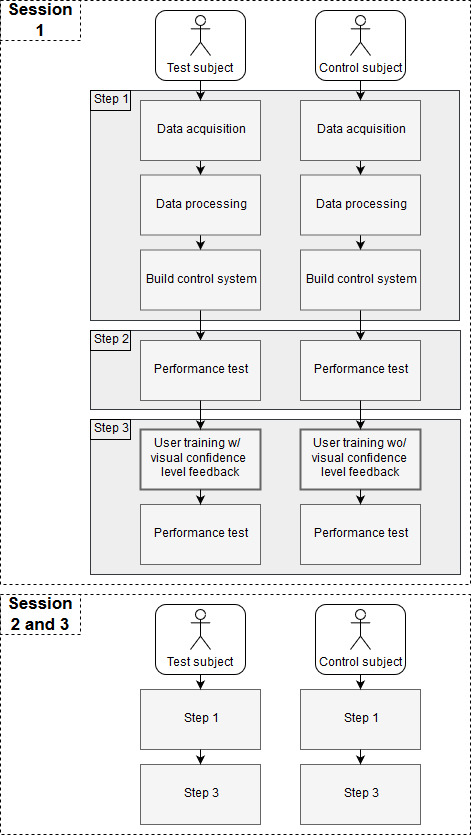
\includegraphics[width=0.64\textwidth]{figures/pMethods/Study_design}  
	\caption{Graphical illustration of the experiment showing the steps of each session for the test and control group. Highlighted is user training in step 3 which is the only procedure that varies between the two groups, and thus the area of research interest in the experiment.}
	\label{fig:std} 
\end{figure}   
